\chapter[Metodologia de Desenvolvimento e Pesquisa]{Metodologia de Desenvolvimento e Pesquisa}

Neste capítulo, estão descritas as estratégias adotadas para o desenvolvimento da pesquisa. O processo foi estruturado em duas etapas principais, que envolvem desde a aquisição e organização dos dados até o treinamento e avaliação dos modelos classificadores, conforme ilustrado na Figura \ref{fig:processometodologico}. 

A primeira etapa consiste na obtenção dos dados por meio de gravações em vídeo do comportamento dos camundongos, dentro do ambiente experimental controlado. A partir das gravações, foram extraídos quadros (\textit{frames}) representativos contendo a região facial dos animais, seguindo os critérios estabelecidos pela \textit{Mouse Grimace Scale} (\acs{MGS}). Em seguida, os \textit{frames} foram armazenados e organizados de acordo com a intensidade de dor atribuída pelos especialistas, dando origem a um conjunto de dados estruturado.

A segunda etapa compreende o pré-processamento das imagens coletadas, incluindo ajustes de formato, padronização e normalização dos dados, de modo a atender aos requisitos de entrada das arquiteturas de redes neurais empregadas. Posteriormente, as imagens foram submetidas às etapas de extração e representação das características relevantes, permitindo que os modelos gerassem saídas probabilísticas associadas às classes de dor previamente definidas.

\begin{figure}[h]
	\centering
	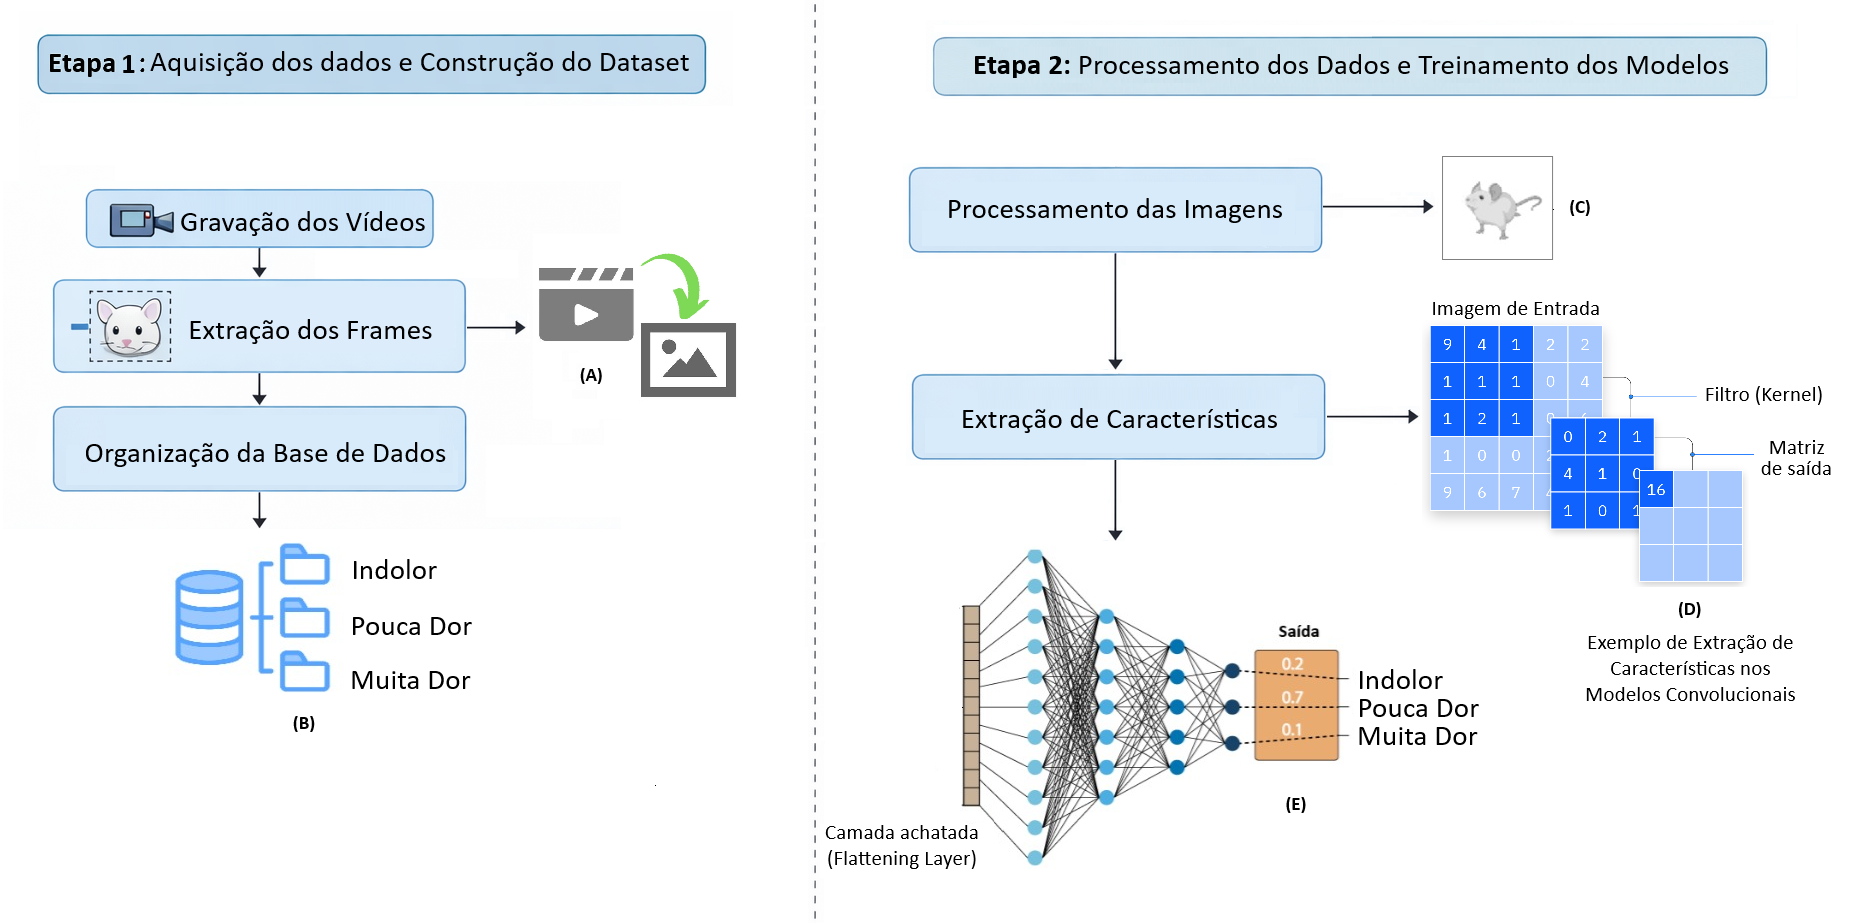
\includegraphics[width=1\linewidth]{figuras/figs_metodologia/Processo_metodologico}
	\caption{Processo metodológico adotado neste estudo. Fonte: o autor.}
	\label{fig:processometodologico}
\end{figure}

\section{Organização e Manejo dos Grupos Experimentais}

Foram utilizados camundongos da espécie \textit{Mus musculus}, modelo animal amplamente empregado em pesquisas biomédicas devido a extensa documentação genética, fisiológica e comportamental disponível na literatura, além de fatores práticos como a alta taxa reprodutiva e facilidade de manejo \cite{Bryda2013}. A amostra foi composta por animais de ambos os sexos, visando aumentar a variabilidade biológica representada no conjunto de dados e minimizar possíveis vieses amostrais. 

Optou-se pela utilização de camundongos isogênicos da linhagem BALB/c em razão de dois fatores principais: (i) a elevada homogeneidade genética característica dos animais isogênicos, reduzindo variabilidades biológicas intragrupo e favorecendo maior controle experimental; e (ii) a coloração clara da pelagem, que proporciona melhor contraste das estruturas faciais nas gravações em vídeo. Esse aspecto é particularmente relevante para a identificação visual de regiões como olhos, orelhas, focinho e vibrissas, facilitando tanto o processo de rotulagem manual quanto a extração automatizada de características associadas às unidades de ação facial descritas pela \acs{MGS}.

Os animais foram alojados em mini-isoladores apropriados, com condições ambientais rigidamente controladas, a fim de minimizar fatores externos capazes de interferir no comportamento espontâneo ou nas expressões faciais. Os camundongos foram mantidos sob ciclo claro/escuro de 12 horas, em ambiente com temperatura controlada (22°C ± 2°C) e umidade relativa de 55\% ± 5\%. A ventilação dos mini-isoladores ocorreu por meio de sistema com filtragem \acs{HEPA}, reduzindo a exposição à agentes externos e contribuindo para maior estabilidade sanitária.

Cada unidade experimental acomodou no máximo cinco animais, respeitando as recomendações institucionais de bem-estar animal e evitando superlotação. Após o período de adaptação ao ambiente experimental, os animais foram distribuídos em dois grupos principais: grupo controle (sem indução de dor) e grupo experimental (submetido ao protocolo de indução nociceptiva). 

As gravações do grupo controle foram utilizadas para caracterizar o padrão basal das expressões faciais. Já as gravações do grupo experimental forneceram amostras visuais das alterações faciais associadas ao estímulo nociceptivo em diferentes momentos temporais, permitindo registrar variações dinâmicas da intensidade de dor ao longo do experimento.

A definição clara das classes e o controle das variáveis experimentais constituem etapas fundamentais para reduzir ruídos no treinamento dos modelos e aumentar a confiabilidade das análises realizadas. Além disso, a estruturação dos grupos permitiu a obtenção de dados longitudinais das expressões faciais, ampliando o potencial exploratório da base de dados e favorecendo o desenvolvimento de modelos mais sensíveis às variações sutis associadas aos diferentes estados fisiológicos avaliados.

\section{Protocolo para Indução de Dor}

Os camundongos pertencentes ao grupo experimental foram submetidos ao modelo clássico de indução da dor via formalina descrito por \cite{Langford2010}. Esse modelo é reconhecido por sua robustez experimental e por produzir respostas fisiológicas e comportamentais previsíveis, tornando-se adequado para investigações envolvendo análise temporal da dor.

O procedimento consiste na administração subcutânea de 20$\mu$L da solução de formalina a 5\% na região plantar da pata traseira direita e produz uma resposta bifásica temporalmente bem definida. Inicialmente, ocorre uma fase aguda (0–15 minutos), correspondente à resposta imediata ao estímulo químico e geralmente associada a maior intensidade dolorosa. Em seguida, desenvolve-se uma segunda fase (15–30 minutos), caracterizada pela manutenção do quadro doloroso em decorrência da ativação de mecanismos inflamatórios locais.

Imediatamente após a aplicação da formalina, os animais foram posicionados nas caixas de observação previamente preparadas para registro em vídeo. As filmagens tiveram início logo após o procedimento, garantindo o registro das alterações faciais correspondentes às fases iniciais do estímulo nociceptivo. Decorridos 30 minutos da injeção, os animais receberam analgesia com sulfato de morfina (5 a 10 mg/kg), administrado por via subcutânea, conforme descrito pela Figura \ref{fig:protocolo}. 

\begin{figure}[h]
	\centering
	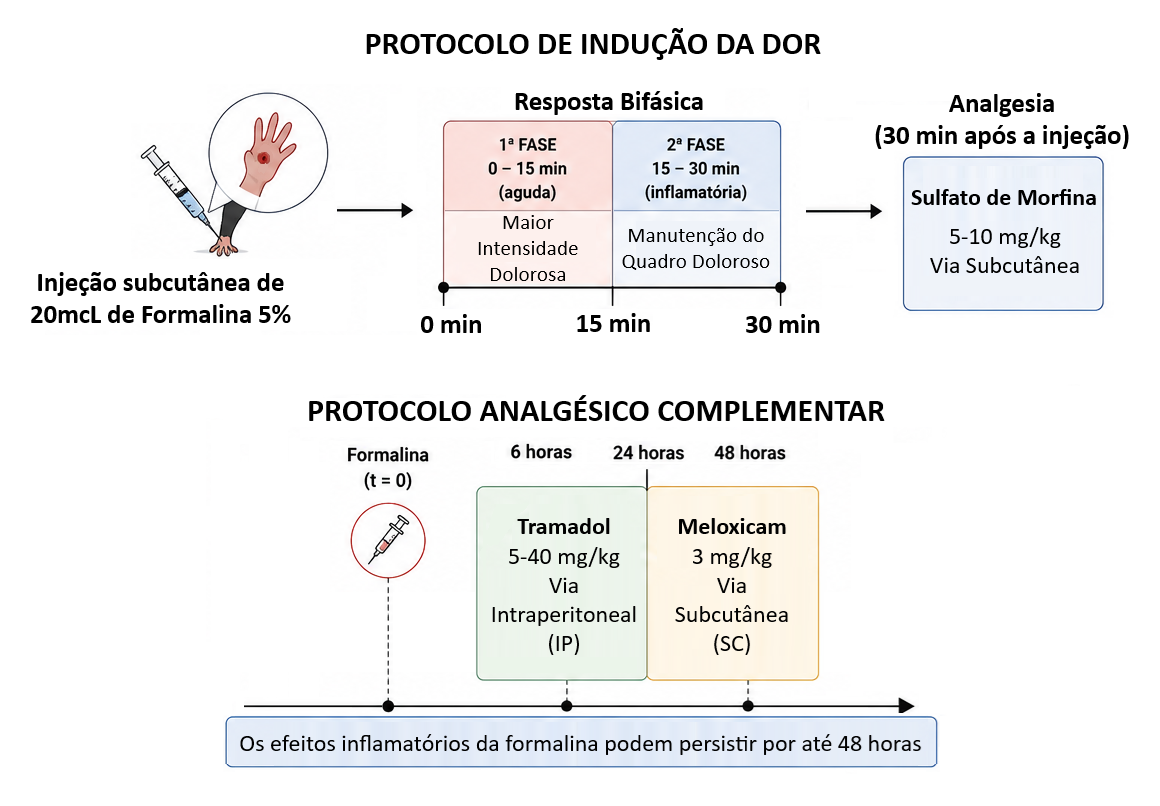
\includegraphics[width=1\linewidth]{figuras/figs_metodologia/langford}
	\caption{Diagrama visual do protocolos experimentais descritos por Langford e Wjeeler-Aceto. Fonte: o autor.}
	\label{fig:protocolo}
\end{figure}

Considerando que os efeitos inflamatórios induzidos pela formalina podem persistir por até 48 horas \cite{WheelerAceto1990}, foi estabelecido um protocolo complementar de controle analgésico e anti-inflamatório. Seis horas após o procedimento inicial, administrou-se cloridrato de tramadol (5–40 mg/kg, via intraperitoneal), repetido também após 24 e 48 horas. Paralelamente, os animais receberam meloxicam (3 mg/kg, via subcutânea) nos mesmos intervalos temporais, com o objetivo de auxiliar no controle do componente inflamatório associado ao procedimento, também descrito pela Figura \ref{fig:protocolo}.

Durante o período total de 72 horas de observação, os animais foram filmados sistematicamente uma hora antes e uma hora após cada administração analgésica. Essa estratégia experimental permitiu registrar diferentes condições fisiológicas: (i) estado basal; (ii) dor ativa sem intervenção imediata; e (iii) dor sob efeito farmacológico. Ao término do período experimental, todos os animais foram submetidos à eutanásia humanitária mediante anestesia profunda com associação de cetamina e xilazina (via intraperitoneal), seguida de deslocamento cervical como método complementar para confirmação do óbito. Todos os procedimentos foram previamente aprovados pelo \ac{CEUA}, em conformidade com as diretrizes do Conselho Nacional de Controle de Experimentação Animal (\acs{CONCEA}/\acs{MCTI}), sob protocolo \textit{\acs{CONCEA}/\acs{MCTI}/0301052024/PESQUISA/000000/2025}.

\section{Aquisição da Base de Dados}

As gravações de ambos os grupos experimentais foram realizadas em alta resolução (4K, 60 quadros por segundo) utilizando câmeras digitais de \textit{smartphones} (modelo \textit{iPhone 13}) previamente higienizados e posicionados frontalmente às caixas de observação. O enquadramento foi ajustado para maximizar a visibilidade dos animais, mantendo distância e ângulo constantes ao longo das sessões.

Cada isolador contendo os camundongos foi filmado durante dois minutos, totalizando 15 repetições por sessão, com intervalos de um minuto entre cada gravação. Esse procedimento foi aplicado tanto antes quanto após o protocolo da indução de dor, assegurando equilíbrio temporal entre as coletas das condições basal e experimental, conforme ilustrado na Figura \ref{fig:capturaimagens}. 

\begin{figure}[h]
	\centering
	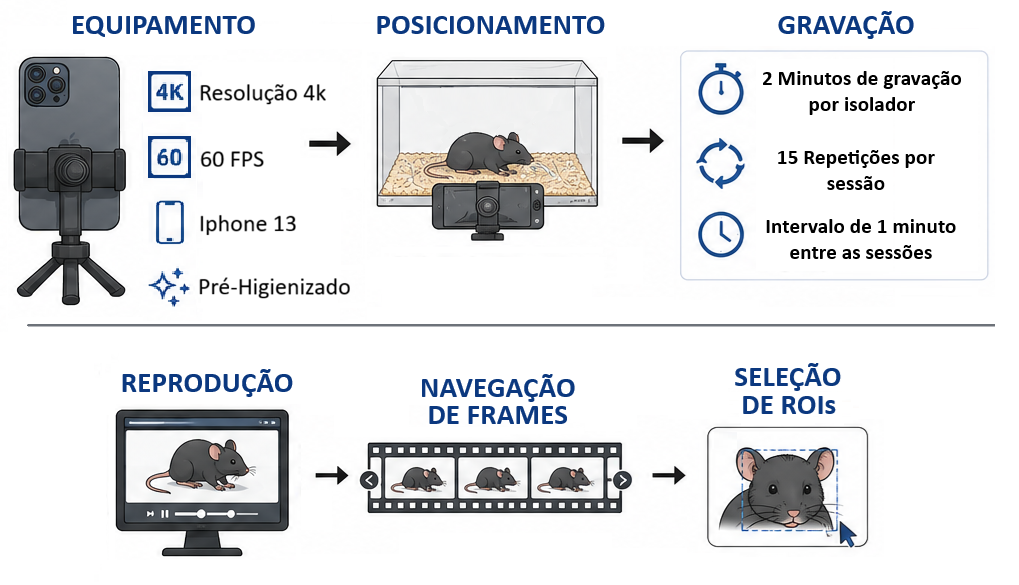
\includegraphics[width=1\linewidth]{figuras/figs_metodologia/captura}
	\caption{Processo de captura dos vídeos para a construção da base de dados. Fonte: Imagem gerada por inteligência artificial (\textit{ChatGPT - OpenAI}), elaborada pelo autor.}
	\label{fig:capturaimagens}
\end{figure}

Após a etapa de captura, os vídeos foram processados por meio de um software desenvolvido especificamente para este estudo, projetado para permitir reprodução controlada dos vídeos, navegação quadro a quadro e seleção manual das regiões de interesse (\acsp{ROI}). Cada imagem extraída foi associada a um identificador único, evitando redundâncias e facilitando o rastreamento posterior das amostras.

Importante destacar que a ferramenta desenvolvida para a extração dos quadros possui um sistema de controle automatizado do armazenamento, o qual impede a duplicidade de imagens na base, além de fornecer ferramentas extras para a inspeção visual e exclusão controlada de quadros inconsistentes ou inadequadas para análise.

Cada imagem selecionada foi inicialmente rotulada em uma das quatro categorias previamente definidas: \textit{Indolor}, \textit{Pouca Dor}, \textit{Muita Dor} ou \textit{Incerto}. A categoria \textit{Incerto} foi utilizada apenas durante o processo inicial de triagem para lidar com imagens ambíguas ou de difícil classificação. 

O software desenvolvido foi disponibilizado à equipe veterinária responsável pela etapa de coleta e rotulagem dos dados. Especialistas com experiência em avaliação de dor em camundongos realizaram a análise visual das imagens utilizando como referência os critérios estabelecidos pela \acs{MGS}. Esse procedimento colaborativo contribuiu para aumentar a confiabilidade da rotulagem e reduzir possíveis vieses individuais.

\section{Seleção das Arquiteturas de Classificação}

A escolha da arquitetura de classificação constitui uma etapa fundamental no desenvolvimento de sistemas computacionais aplicados à análise de imagens. A definição do modelo impacta diretamente as tarefas supervisionadas de classificação dos padrões visuais, influenciando aspectos como desempenho preditivo, estabilidade do treinamento, capacidade de generalização e custo computacional.

Com o objetivo de fundamentar essa escolha de forma criteriosa, foi conduzida uma revisão da literatura especializada envolvendo trabalhos clássicos e recentes nas áreas de aprendizado profundo, reconhecimento facial e classificação de imagens. Os principais critérios considerados para seleção das arquiteturas incluíram: (i) desempenho reportado na literatura; (ii) eficiência computacional; (iii) capacidade de aprendizado e generalização; e (iv) potencial de aplicação em cenários com restrições computacionais.

Dentre as arquiteturas selecionadas, destacam-se inicialmente os modelos baseados em Redes Neurais Convolucionais (\acsp{CNN}), amplamente consolidados em tarefas de visão computacional devido à elevada capacidade de extração automática das características espaciais.

A família de arquiteturas \textit{ResNet} foi incluída neste estudo em razão de seu desempenho amplamente validado em \textit{benchmarks} de larga escala, como o \textit{ImageNet}. Seu principal diferencial está na incorporação do aprendizado residual, permitindo o treinamento de redes profundas com maior estabilidade e reduzindo problemas associados ao desaparecimento do gradiente. Além disso, sua estrutura modular possibilita a utilização de variantes com diferentes profundidades, tornando a arquitetura flexível para distintos cenários computacionais.

Outra arquitetura baseada em \acs{CNN} considerada neste trabalho foi a \textit{DenseNet}, caracterizada pelo padrão de conectividade densa entre suas camadas. Nesse modelo, cada camada recebe como entrada os mapas de características produzidos por todas as camadas anteriores dentro do mesmo bloco, promovendo reaproveitamento contínuo das informações ao longo da rede. Em problemas que envolvem padrões visuais sutis — como os indicadores faciais associados à \acs{MGS} —, essa capacidade de preservação e combinação de informações em diferentes níveis de abstração pode favorecer a construção de representações mais discriminativas.

A arquitetura \textit{MobileNet} também foi selecionada devido à sua elevada eficiência computacional, sendo projetada especificamente para aplicações com restrições de processamento. Seu principal diferencial consiste na utilização de convoluções separáveis em profundidade, reduzindo significativamente o número de parâmetros e o custo computacional sem comprometer substancialmente o desempenho. Além disso, mecanismos como o \textit{width multiplier} e o \textit{resolution multiplier} permitem ajustar diretamente o equilíbrio entre desempenho e complexidade computacional, ampliando o potencial de aplicação em dispositivos móveis e sistemas embarcados.

Além das arquiteturas convolucionais tradicionais, este estudo também investigou abordagens baseadas em mecanismos de atenção por meio da arquitetura \textit{Vision Transformer} (\acs{VIT}). Diferentemente das \acsp{CNN}, o \acs{VIT} processa imagens utilizando mecanismos de autoatenção, possibilitando modelar dependências globais entre diferentes regiões da imagem desde as etapas iniciais do treinamento.

A adoção do \acs{VIT} foi motivada pela capacidade de capturar relações de longo alcance entre diferentes regiões faciais, potencialmente favorecendo representações mais abrangentes dos padrões associados à dor. Essa característica torna a arquitetura particularmente interessante em problemas envolvendo variações sutis nas expressões faciais, nos quais relações espaciais globais podem desempenhar papel relevante na discriminação entre diferentes níveis de dor.

Entretanto, diferentemente das arquiteturas convolucionais, modelos baseados em \textit{Transformers} tendem a demandar maior volume de dados para treinamento eficiente, uma vez que não incorporam explicitamente os vieses indutivos locais característicos das \acsp{CNN}. Dessa forma, sua inclusão neste estudo também permitiu investigar o impacto dessas diferenças estruturais em cenários associados ao uso de \textit{transfer learning}.

A seleção conjunta dessas arquiteturas possibilitou estabelecer uma análise comparativa entre modelos baseados em diferentes paradigmas de aprendizado visual, permitindo investigar não apenas o desempenho preditivo, mas também características relacionadas à eficiência computacional, capacidade de generalização e adequação ao problema proposto.

\section{Configuração Experimental}

Em problemas relacionados ao aprendizado supervisionado, pequenas variações na organização das amostras, nos procedimentos de pré-processamento ou na divisão entre os conjuntos de treinamento e validação podem influenciar significativamente os resultados obtidos, comprometendo a reprodutibilidade e a comparabilidade dos experimentos. Portanto, a seguinte seção tem como objetivo descrever as configurações utilizadas para o processamento dos dados, bem como condução metodológica dos experimentos.

Visando promover a transparência científica e favorecer a reprodução dos experimentos conduzidos nesta pesquisa, todos os recursos desenvolvidos foram disponibilizados publicamente por meio de repositórios digitais. Em particular, foram compartilhados: (i) o código-fonte da ferramenta desenvolvida para a extração, organização e gerenciamento da base de dados; (ii) o projeto contendo a implementação dos modelos de aprendizado profundo, bem como as rotinas de treinamento, validação e avaliação experimental; e (iii) a base de dados construída e utilizada ao longo deste trabalho. Todos esses recursos encontram-se disponíveis no repositório oficial do autor, acessível em:

\begin{itemize}
	
	\item Ferramenta para geração da base de dados:\\
	\url{https://github.com/Marcio-Salmazo/Projeto-video-player}
	
	\item Implementação dos modelos classificadores:\\
	\url{https://github.com/Marcio-Salmazo/Projeto-Classificadores}
	
	\item Base de dados utilizada nesta pesquisa:\\
	\url{https://github.com/Marcio-Salmazo/Dataset-MGS}
	
\end{itemize}

\subsection*{Preparação da Base de Dados}

O controle sobre a preparação da base de dados foi aplicado por meio de um \textit{Script} em \textit{python}, desenvolvido para gerenciar a separação automatizada da base em subconjuntos de treinamento e validação. O algoritmo permite definir previamente a proporção de imagens destinada a cada subconjunto, reproduzindo automaticamente a estrutura hierárquica das classes em cada diretório e preservando a integridade do conjunto original de dados.

O processo de divisão da base foi realizado de forma estratificada por classe, assegurando a manutenção proporcional das categorias entre os subconjuntos gerados. Para cada classe, o algoritmo aplica um processo de embaralhamento pseudoaleatório controlado por uma semente fixa (\textit{random seed}), garantindo reprodutibilidade experimental em diferentes execuções. Após o embaralhamento, as imagens são copiadas da base original e redistribuídas automaticamente entre os subconjuntos definidos. A estrutura final da base de dados é apresentada na Figura \ref{fig:estrutrabase}.

\begin{figure}[h]
	\centering
	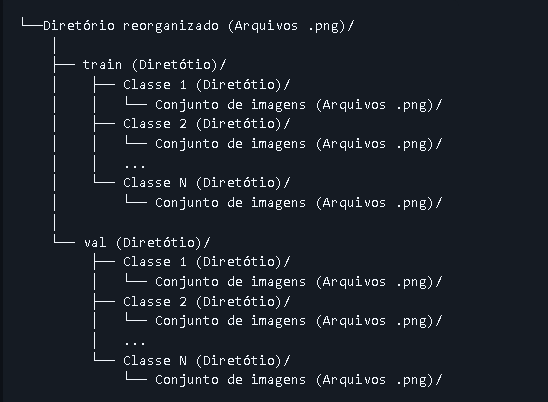
\includegraphics[width=.8\linewidth]{figuras/figs_metodologia/estrutra_base}
	\caption{Estrutura final da base de dados, após o processo de divisão dos conjuntos de treino e validação. Fonte: o autor.}
	\label{fig:estrutrabase}
\end{figure}

% TRECHO NOVO SOBRE O CARREGAMENTO DOS DADOS
\subsection*{Carregamento dos Dados}

Após a organização da base de dados, foi aplicada uma etapa de pré-processamento com o objetivo de padronizar as imagens e proporcionar condições adequadas para o treinamento das arquiteturas investigadas. Nessa etapa, foram adotadas estratégias distintas para os conjuntos de treinamento e validação, de forma a preservar as características específicas de cada etapa do processo de aprendizado.

Para o conjunto de treinamento, empregou-se uma estratégia de \textit{data augmentation} leve, baseada em pequenas transformações geométricas e espaciais realizadas de forma aleatória. Essas modificações tiveram como finalidade ampliar artificialmente a variabilidade das amostras disponíveis, expondo os modelos a diferentes representações de uma mesma imagem sem alterar as características faciais associadas à expressão de dor. Essa abordagem contribui para a capacidade de generalização dos classificadores diante de pequenas variações presentes durante a aquisição das imagens.

Em contrapartida, o conjunto de validação foi submetido apenas a operações de padronização, sem a aplicação de transformações aleatórias. Essa estratégia garante que o desempenho dos modelos seja avaliado de maneira consistente ao longo do treinamento, permitindo comparações imparciais entre as diferentes arquiteturas investigadas. Por fim, todas as imagens foram normalizadas antes de serem utilizadas pelos modelos, assegurando uma representação padronizada dos dados e contribuindo para a estabilidade do processo de treinamento.

\subsection*{Métricas para Avaliação do Desempenho}

Durante o treino, métricas primárias como função de perda (\textit{loss}) e acurácia (\textit{accuracy}) foram registradas automaticamente ao final de cada época por meio dos mecanismos de \textit{log} integrados ao \textit{TensorFlow} e às rotinas implementadas em ambiente \textit{JAX/Flax}. Esses registros foram armazenados em arquivos nos formatos \textit{.csv} e \textit{.xlsx}, possibilitando posterior organização, consolidação e análise dos resultados obtidos.

A acurácia foi utilizada como principal indicador de desempenho dos classificadores por representar a proporção de amostras corretamente classificadas em relação ao total avaliado. Considerando que o objetivo central deste estudo consiste na comparação da capacidade de diferentes arquiteturas neurais em identificar padrões faciais associados à dor, a acurácia fornece uma medida direta e intuitiva da eficiência global dos modelos. 

De modo complementar, a função de perda foi utilizada como principal métrica para acompanhamento do processo de otimização durante o treinamento. Diferentemente da acurácia, a função de perda quantifica o grau de erro cometido pelo modelo em suas predições, considerando também o nível de confiança associado às decisões produzidas. Dessa forma, reduções sucessivas nos valores de perda indicam que o modelo está ajustando seus parâmetros internos de maneira consistente, aproximando suas previsões dos rótulos esperados e favorecendo o processo de convergência.

Embora a literatura apresente diversas métricas complementares para avaliação de classificadores, tais como precisão, sensibilidade (\textit{recall}), \textit{F1-score} e matrizes de confusão, sua utilização não foi considerada necessária para os objetivos deste estudo. Como a pesquisa teve como foco principal a análise comparativa da eficiência de diferentes arquiteturas de aprendizado profundo, priorizou-se a utilização de métricas capazes de representar diretamente o desempenho global e a dinâmica de aprendizado dos modelos. Dessa forma, acurácia e função de perda mostraram-se suficientes para sustentar as análises realizadas e responder às questões de pesquisa propostas.

% TRECHO NOVO SOBRE O DETALHAMENTO DE HARDWARE
\subsection*{Detalhamento de Hardware}

Os experimentos conduzidos nesta pesquisa foram realizados em dois ambientes computacionais distintos, de acordo com as exigências de processamento de cada arquitetura investigada. Os treinamentos envolvendo as arquiteturas convolucionais foram executados em uma estação de trabalho pessoal equipada com processador \textit{AMD Ryzen 7 5700X}, 24 GB de memória \textit{RAM} e uma unidade de processamento gráfico (GPU) \textit{NVIDIA GeForce RTX 3070}. Cabe destacar que os modelos avaliados apresentam complexidade computacional compatível com a capacidade de processamento e memória disponibilizadas pela GPU.

Por outro lado, os experimentos envolvendo a arquitetura \acs{VIT} foram conduzidos em um servidor remoto pertencente à Universidade Federal de Uberlândia (UFU), acessado por meio do protocolo SSH. O servidor utilizado foi equipada com processador \textit{Intel Xeon Gold 6426Y}, 256 GB de memória \textit{RAM} e uma GPU \textit{NVIDIA Ampere A40}, com 48GB de \textit{VRAM}. A utilização dessa infraestrutura foi necessária ao maior custo computacional associado aos mecanismos de autoatenção empregados pelos modelos baseados em \textit{Transformers}, os quais apresentam maior consumo de memória e maior tempo de processamento durante o treinamento, mesmo com a utilização de \textit{transfer learning} para reduzir a demanda por recursos computacionais.
